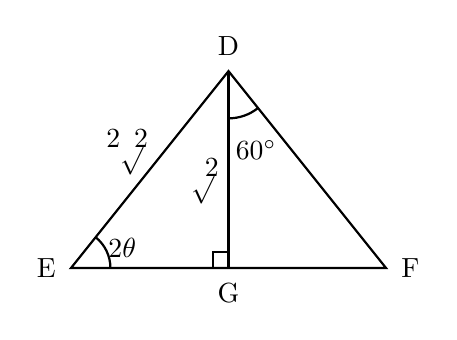
\begin{tikzpicture}[scale=1]

    % Define the vertices of the triangles
    \coordinate (G) at (0,0);
    \coordinate (E) at (-2,0);
    \coordinate (F) at (2,0);
    \coordinate (D) at (0,2.5);

    % Draw the main triangle EDF
    \draw[thick] (E) -- (F) -- (D) -- cycle;

    % Draw the altitude DG
    \draw[thick] (D) -- (G);

    % Draw the right-angle symbol at G
    \draw[thick] (G) ++(-0.2,0) -- ++(0,0.2) -- ++(0.2,0);

    % Draw the angle arcs
    % Arc at E
    \draw[thick] (E) ++(0:0.5) arc (0:51.3:0.5);
    % Arc at D inside triangle DGF
    \draw[thick] (D) ++(270:0.6) arc (270:308.6:0.6);

    % Add labels for the points
    \node[below, yshift=-2pt] at (G) {G};
    \node[left, xshift=-2pt] at (E) {E};
    \node[right, xshift=2pt] at (F) {F};
    \node[above, yshift=2pt] at (D) {D};

    % Add length labels (using \surd without the top bar and repositioned)
    \node[above left] at (-0.9, 1.05) {$2$\raisebox{-7.5pt}{$\surd$}$\!\!2$};
    \node[left] at (0, 1.1) {\raisebox{-7.5pt}{$\surd$}$\!\!2$};

    % Add angle labels
    \node at (-1.35, 0.25) {$2\theta$};
    % Rotate the 60 degree text to match the image visually
    \node at (0.35, 1.5) {$60^{\circ}$};

\end{tikzpicture}